\documentclass[tikz,border=8pt]{standalone}
% Shared look for every TikZ diagram. Load with \input{../../tools/tikz-style.tex}
\usepackage[T1]{fontenc}
\usepackage{lmodern}
\renewcommand{\sfdefault}{lmr}  % diagrams use the same serif as the text
\usetikzlibrary{arrows.meta, positioning, shapes.geometric, calc, fit, backgrounds}
\definecolor{cblue}{HTML}{4C78A8}
\definecolor{corange}{HTML}{F58518}
\definecolor{cgreen}{HTML}{54A24B}
\definecolor{cred}{HTML}{E45756}
\definecolor{cpurple}{HTML}{B279A2}
\definecolor{cgrey}{HTML}{6B6B6B}
\tikzset{
  every picture/.style={font=\sffamily, line width=1.2pt},
  box/.style={draw=#1, fill=#1!12, rounded corners=4pt, align=center, inner sep=7pt, minimum height=1.1cm},
  box/.default=cgrey,
  arrow/.style={-{Stealth[length=3mm]}, draw=cgrey, line width=1.4pt},
  title/.style={font=\sffamily\bfseries\Large},
  note/.style={font=\sffamily\small, text=cgrey, align=center},
}
\AtBeginDocument{\hyphenpenalty=10000 \exhyphenpenalty=10000}

\begin{document}
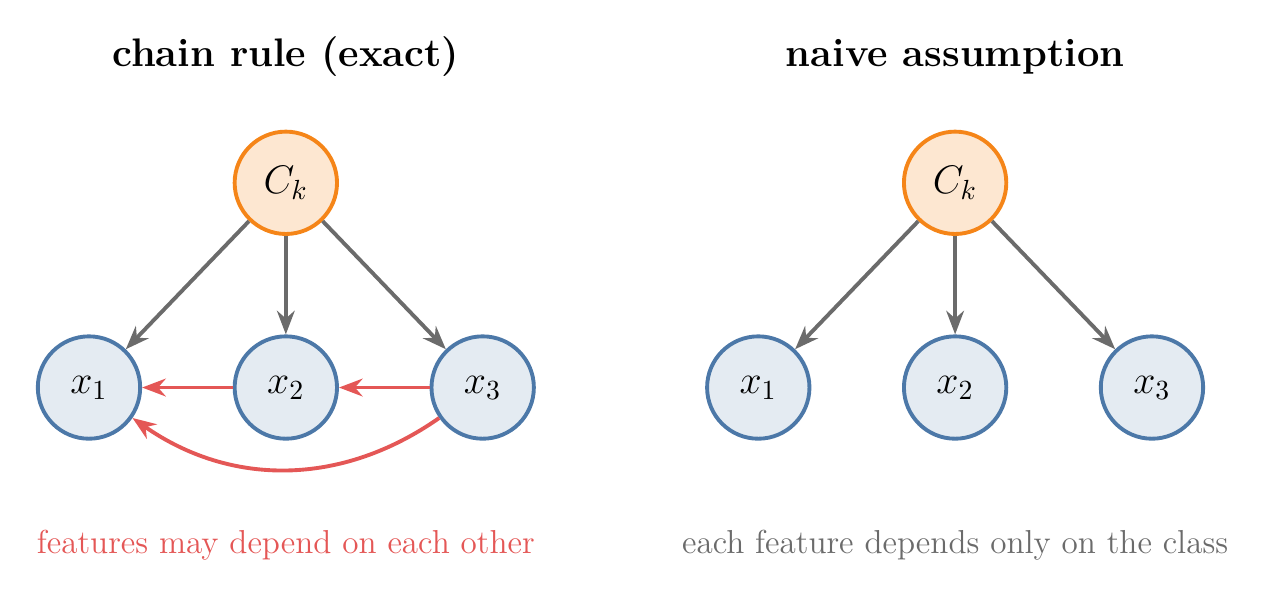
\begin{tikzpicture}[every node/.append style={font=\sffamily\Large},
    cls/.style={circle, draw=corange, fill=corange!20, minimum size=1.3cm, line width=1.4pt},
    ft/.style={circle, draw=cblue, fill=cblue!15, minimum size=1.3cm, line width=1.4pt},
    dep/.style={-{Stealth[length=3mm]}, draw=cgrey, line width=1.4pt},
    link/.style={-{Stealth[length=3mm]}, draw=cred, line width=1.4pt}]
  \begin{scope}
    \node[title] at (2.5,2.6) {chain rule (exact)};
    \node[cls] (c) at (2.5,1) {$C_k$};
    \node[ft] (x1) at (0,-1.6) {$x_1$};
    \node[ft] (x2) at (2.5,-1.6) {$x_2$};
    \node[ft] (x3) at (5,-1.6) {$x_3$};
    \foreach \x in {x1,x2,x3} \draw[dep] (c) -- (\x);
    \draw[link] (x2) -- (x1);
    \draw[link] (x3) -- (x2);
    \draw[link] (x3) to[bend left=35] (x1);
    \node[font=\sffamily\large, text=cred] at (2.5,-3.6) {features may depend on each other};
  \end{scope}
  \begin{scope}[xshift=8.5cm]
    \node[title] at (2.5,2.6) {naive assumption};
    \node[cls] (c) at (2.5,1) {$C_k$};
    \node[ft] (x1) at (0,-1.6) {$x_1$};
    \node[ft] (x2) at (2.5,-1.6) {$x_2$};
    \node[ft] (x3) at (5,-1.6) {$x_3$};
    \foreach \x in {x1,x2,x3} \draw[dep] (c) -- (\x);
    \node[font=\sffamily\large, text=cgrey] at (2.5,-3.6) {each feature depends only on the class};
  \end{scope}
\end{tikzpicture}
\end{document}
